% =============================================================================
% Binary Skin Cancer Classification with Fine-Tuning
% Machine Learning — Final Project Paper
% =============================================================================
\documentclass[11pt, a4paper, twocolumn]{article}

% --- Packages ---
\usepackage[utf8]{inputenc}
\usepackage[T1]{fontenc}
\usepackage[english]{babel}
\usepackage{amsmath, amssymb}
\usepackage{graphicx}
\usepackage{booktabs}
\usepackage{caption}
\usepackage{subcaption}
\usepackage{hyperref}
\usepackage{listings}
\usepackage{xcolor}
\usepackage[margin=2cm]{geometry}
\usepackage{float}
\usepackage{enumitem}
\usepackage{algorithm}
\usepackage{algorithmic}
\usepackage{multirow}
\usepackage{array}

% --- Code listing style ---
\definecolor{codebg}{rgb}{0.95, 0.95, 0.95}
\definecolor{codegreen}{rgb}{0.0, 0.5, 0.0}
\definecolor{codegray}{rgb}{0.5, 0.5, 0.5}
\definecolor{codepurple}{rgb}{0.58, 0.0, 0.82}
\lstset{
    backgroundcolor=\color{codebg},
    basicstyle=\ttfamily\scriptsize,
    keywordstyle=\color{codepurple}\bfseries,
    commentstyle=\color{codegreen},
    stringstyle=\color{red!60!black},
    numberstyle=\tiny\color{codegray},
    breaklines=true,
    frame=single,
    numbers=left,
    numbersep=5pt,
    language=Python,
    captionpos=b,
    tabsize=4,
}

% --- Hyperlinks ---
\hypersetup{
    colorlinks=true,
    linkcolor=blue!70!black,
    citecolor=blue!70!black,
    urlcolor=blue!70!black,
}

% =============================================================================
\title{
    \textbf{Binary Skin Cancer Classification via Fine-Tuning:\\
    A Comparative Study of ResNet-50, EfficientNetV2-S, and ViT-B/16}
}
\author{
    Gerardo Macias Romo\\[2pt]
    \textit{Universidad Panamericana}\\[2pt]
    \textit{Machine Learning 2 --- 8th Semester}\\[2pt]
    \texttt{geras.4215@gmail.com}
}
\date{May 2026}

\begin{document}
\maketitle

% =============================================================================
\begin{abstract}
Skin cancer is one of the most prevalent types of cancer worldwide,
and early detection is critical for patient survival. This work presents
a comparative study of three deep learning architectures ---
ResNet-50, EfficientNetV2-S, and ViT-B/16 --- for binary classification
of dermoscopic skin lesion images as malignant or benign.
All models are fine-tuned from ImageNet-pretrained weights on the
ISIC 2024 SLICE-3D Permissive dataset, which exhibits extreme class
imbalance (99.87\% benign vs.\ 0.13\% malignant). We employ a
multi-pronged strategy combining weighted random sampling,
cost-sensitive loss functions, data augmentation, mixed-precision
training, and gradient clipping. Our results demonstrate that all three
architectures achieve strong discriminative performance, with
ViT-B/16 reaching a peak validation AUC-ROC of 0.95 and
EfficientNetV2-S achieving the most consistent performance with
an AUC-ROC of 0.94. The findings confirm that transfer learning
is an effective approach for medical image classification even under
severe resource and data constraints.
\end{abstract}

\textbf{Keywords:} skin cancer, melanoma detection, transfer learning,
fine-tuning, deep learning, class imbalance, ResNet, EfficientNet,
Vision Transformer, ISIC 2024.

% =============================================================================
\section{Introduction}
\label{sec:introduction}

Skin cancer represents one of the most common forms of cancer globally,
with melanoma being the deadliest variant, accounting for approximately
75\% of skin cancer-related deaths despite representing only about 1\%
of skin cancer diagnoses \cite{siegel2023}. Early detection through
dermoscopic image analysis has been shown to significantly improve
prognosis, motivating the development of computer-aided diagnosis (CAD)
systems.

Deep learning has revolutionized medical image classification, with
convolutional neural networks (CNNs) and more recently Vision
Transformers achieving dermatologist-level performance on skin lesion
classification tasks \cite{esteva2017, dosovitskiy2021}. Transfer
learning --- where models pretrained on large-scale datasets such as
ImageNet are adapted to domain-specific tasks --- has become the
standard approach, particularly when labeled medical data is scarce
or highly imbalanced \cite{he2016, tan2021}.

In this work, we present a comparative study of three state-of-the-art
architectures for binary classification of skin lesions:

\begin{enumerate}[noitemsep]
    \item \textbf{ResNet-50} \cite{he2016}: A classic residual CNN
          with skip connections that enable training of very deep networks.
    \item \textbf{EfficientNetV2-S} \cite{tan2021}: An optimized CNN
          designed via Neural Architecture Search (NAS) with compound
          scaling of depth, width, and resolution.
    \item \textbf{ViT-B/16} \cite{dosovitskiy2021}: A Vision Transformer
          that applies the self-attention mechanism to sequences of
          image patches.
\end{enumerate}

All models are fine-tuned on the ISIC 2024 SLICE-3D Permissive dataset
\cite{isic2024}, which presents a significant challenge due to its
extreme class imbalance: only 0.13\% of images are malignant. We
address this challenge through a combination of sampling strategies,
cost-sensitive learning, and data augmentation techniques.

% =============================================================================
\section{Dataset}
\label{sec:dataset}

\subsection{ISIC 2024 SLICE-3D Permissive}

The International Skin Imaging Collaboration (ISIC) 2024 dataset is a
large-scale collection of dermoscopic images released under a CC-BY 4.0
license. Table~\ref{tab:dataset_overview} summarizes the dataset
characteristics.

\begin{table}[H]
    \centering
    \caption{Dataset overview.}
    \label{tab:dataset_overview}
    \begin{tabular}{@{}ll@{}}
        \toprule
        \textbf{Property} & \textbf{Value} \\
        \midrule
        Total images       & 217,477 \\
        Malignant          & 294 (0.13\%) \\
        Benign             & 217,183 (99.87\%) \\
        Resolution         & $\sim$128$\times$128 px (variable) \\
        Format             & JPEG, RGB \\
        License            & CC-BY 4.0 \\
        \bottomrule
    \end{tabular}
\end{table}

The dataset exhibits an \textbf{extreme class imbalance} with a ratio
of approximately 739:1 (benign to malignant), making it one of the most
challenging binary classification settings in medical imaging. This
imbalance ratio means that a naive classifier predicting all images as
benign would achieve 99.87\% accuracy while failing to detect any
malignant cases.

\subsection{Exploratory Data Analysis}

Our exploratory analysis revealed the following characteristics:

\begin{itemize}[noitemsep]
    \item Image resolutions are relatively uniform around
          $128 \times 128$ pixels, with minor variations.
    \item Visual differences between benign and malignant lesions are
          subtle and often indistinguishable to the untrained eye.
    \item Color distributions vary across samples due to differences
          in skin tone, lighting, and imaging equipment.
\end{itemize}

% =============================================================================
\section{Methodology}
\label{sec:methodology}

\subsection{Data Preparation}

\subsubsection{Stratified Split}

The dataset was divided using stratified sampling to preserve the
class distribution across splits:

\begin{table}[H]
    \centering
    \caption{Data split configuration.}
    \label{tab:splits}
    \begin{tabular}{@{}lccc@{}}
        \toprule
        \textbf{Split} & \textbf{Ratio} & \textbf{Malignant} & \textbf{Benign (subset)} \\
        \midrule
        Train & 70\% & $\sim$205 & 10,000 \\
        Val   & 15\% & $\sim$44  & 2,000 \\
        Test  & 15\% & $\sim$44  & 5,000 \\
        \bottomrule
    \end{tabular}
\end{table}

To enable feasible training times on a single GPU, we employed
\textbf{subset sampling}: all malignant samples were retained while
a random subset of benign samples was drawn for each split. This
strategy preserves every positive example while reducing computational
cost.

\subsubsection{Data Augmentation}

Training images were augmented using the following transformations,
applied on-the-fly during training:

\begin{itemize}[noitemsep]
    \item Resize to $224 \times 224$ pixels
    \item Random horizontal flip ($p = 0.5$)
    \item Random vertical flip ($p = 0.5$)
    \item Random rotation ($\pm 15^{\circ}$)
    \item Color jitter (brightness $\pm 0.2$, contrast $\pm 0.2$,
          saturation $\pm 0.2$, hue $\pm 0.05$)
    \item ImageNet normalization ($\mu = [0.485, 0.456, 0.406]$,
          $\sigma = [0.229, 0.224, 0.225]$)
\end{itemize}

Validation and test images received only resizing and normalization
(no augmentation) to ensure deterministic evaluation.

\subsection{Class Imbalance Handling}
\label{subsec:imbalance}

We employed a three-pronged strategy to address the extreme class
imbalance:

\begin{enumerate}[noitemsep]
    \item \textbf{WeightedRandomSampler:} Each training sample was
          assigned a sampling weight inversely proportional to its
          class frequency, effectively creating balanced mini-batches
          with approximately 50\% positive and 50\% negative samples.
          The weight for class $c$ is defined as:
          \begin{equation}
              w_c = \frac{1}{N_c}
          \end{equation}
          where $N_c$ is the number of samples in class $c$.

    \item \textbf{Cost-sensitive loss:} We used Binary Cross-Entropy
          with Logits Loss with a \texttt{pos\_weight} parameter:
          \begin{equation}
              \text{pos\_weight} = \frac{N_{\text{neg}}}{N_{\text{pos}}}
              \approx 48.8
          \end{equation}
          This penalizes false negatives approximately 49 times more
          than false positives, reflecting the clinical importance of
          not missing malignant cases.

    \item \textbf{Subset sampling:} As described above, retaining all
          positives while subsampling negatives reduces the effective
          imbalance ratio from 739:1 to approximately 49:1.
\end{enumerate}

\subsection{Model Architectures}
\label{subsec:models}

All three models were loaded with pretrained ImageNet weights and their
classification heads were replaced with a single output neuron for
binary classification via sigmoid activation.

\subsubsection{ResNet-50}

ResNet-50 \cite{he2016} is a 50-layer deep residual network with
25.6M parameters. The key innovation is the use of \textit{skip
connections} (identity shortcuts) that allow gradients to flow
directly through the network, enabling training of very deep
architectures. The final fully-connected layer
(\texttt{model.fc}) was replaced with a linear layer mapping from
2,048 features to 1 output.

\subsubsection{EfficientNetV2-S}

EfficientNetV2-S \cite{tan2021} is an optimized CNN with 21.5M
parameters, designed using Neural Architecture Search (NAS). It
employs \textit{compound scaling} to jointly optimize network depth,
width, and input resolution. The model uses Fused-MBConv blocks in
early layers and standard MBConv blocks in later layers. The
classifier head (\texttt{model.classifier[1]}) was replaced with
a linear layer mapping from 1,280 features to 1 output.

\subsubsection{ViT-B/16}

The Vision Transformer Base with 16$\times$16 patches (ViT-B/16)
\cite{dosovitskiy2021} contains 86.6M parameters. It divides each
$224 \times 224$ input image into a sequence of $14 \times 14 = 196$
non-overlapping patches of size $16 \times 16$, which are linearly
projected into embedding vectors. A learnable \texttt{[CLS]} token is
prepended, and the sequence is processed by 12 Transformer encoder
layers with multi-head self-attention. The classification head
(\texttt{model.heads.head}) was replaced with a linear layer mapping
from 768 features to 1 output.

\begin{table}[H]
    \centering
    \caption{Model comparison.}
    \label{tab:models}
    \begin{tabular}{@{}lcr@{}}
        \toprule
        \textbf{Model} & \textbf{Type} & \textbf{Parameters} \\
        \midrule
        ResNet-50        & Residual CNN  & 25.6 M \\
        EfficientNetV2-S & NAS-designed CNN & 21.5 M \\
        ViT-B/16         & Vision Transformer & 86.6 M \\
        \bottomrule
    \end{tabular}
\end{table}

\subsection{Training Configuration}
\label{subsec:training}

Table~\ref{tab:hyperparams} summarizes the training hyperparameters
used for all three models.

\begin{table}[H]
    \centering
    \caption{Training hyperparameters.}
    \label{tab:hyperparams}
    \begin{tabular}{@{}ll@{}}
        \toprule
        \textbf{Hyperparameter} & \textbf{Value} \\
        \midrule
        Epochs          & 10 \\
        Batch size      & 64 \\
        Optimizer       & AdamW \\
        Backbone LR     & $1 \times 10^{-4}$ \\
        Head LR         & $1 \times 10^{-3}$ \\
        Weight decay    & $1 \times 10^{-4}$ \\
        Gradient clipping & max\_norm = 1.0 \\
        Precision       & Mixed (FP16 via AMP) \\
        Loss            & BCEWithLogitsLoss \\
        pos\_weight     & $N_{\text{neg}} / N_{\text{pos}} \approx 48.8$ \\
        \bottomrule
    \end{tabular}
\end{table}

\subsubsection{Differential Learning Rates}

We used \textbf{differential learning rates}, assigning a lower
learning rate ($10^{-4}$) to the pretrained backbone layers and a
higher learning rate ($10^{-3}$) to the randomly initialized
classification head. This strategy preserves the learned feature
representations while allowing the head to adapt quickly to the
new task.

\subsubsection{Mixed Precision Training}

To maximize GPU memory efficiency on our 8~GB VRAM budget, we employed
\textbf{Automatic Mixed Precision (AMP)} via PyTorch's
\texttt{torch.amp.autocast} and \texttt{GradScaler}. This performs
forward and backward passes in FP16 while maintaining FP32 master
weights, reducing memory consumption by approximately 50\% and
accelerating computation through the GPU's Tensor Cores.

\subsubsection{Gradient Clipping and NaN Protection}

The combination of high \texttt{pos\_weight} ($\approx 49$) and FP16
arithmetic can cause gradient explosion, leading to NaN values in
model weights. We addressed this with two safeguards:

\begin{enumerate}[noitemsep]
    \item \textbf{Gradient clipping:} Applied
          \texttt{clip\_grad\_norm\_(max\_norm=1.0)} after unscaling
          gradients but before the optimizer step.
    \item \textbf{NaN sanitization:} Applied
          \texttt{torch.nan\_to\_num()} on output logits during
          evaluation, replacing NaN with 0, $+\infty$ with 10, and
          $-\infty$ with $-10$.
\end{enumerate}

\subsubsection{Model Selection}

The best model checkpoint was saved based on the highest validation
AUC-ROC observed during training. After training, the best weights
were reloaded for final test-set evaluation.

% =============================================================================
\section{Training Procedure}
\label{sec:training_procedure}

Algorithm~\ref{alg:training} describes the complete training loop
used for each model.

\begin{algorithm}[H]
    \caption{Fine-tuning training loop}
    \label{alg:training}
    \begin{algorithmic}[1]
        \REQUIRE Model $M$, train loader $\mathcal{D}_{\text{train}}$,
                 val loader $\mathcal{D}_{\text{val}}$, epochs $E$
        \STATE Initialize optimizer (AdamW, differential LR)
        \STATE Initialize GradScaler for AMP
        \STATE best\_auc $\leftarrow 0$
        \FOR{epoch $= 1$ to $E$}
            \STATE $M$.train()
            \FOR{each batch $(X, y) \in \mathcal{D}_{\text{train}}$}
                \STATE Forward pass in FP16: $\hat{y} = M(X)$
                \STATE Compute loss: $\mathcal{L} = \text{BCE}(\hat{y}, y)$
                \STATE Backward pass with scaled gradients
                \STATE Unscale gradients
                \STATE Clip gradients: $\|\nabla\| \leq 1.0$
                \STATE Optimizer step + scaler update
            \ENDFOR
            \STATE Evaluate on $\mathcal{D}_{\text{val}}$
            \IF{val\_auc $>$ best\_auc}
                \STATE Save model checkpoint
                \STATE best\_auc $\leftarrow$ val\_auc
            \ENDIF
        \ENDFOR
        \STATE Load best checkpoint
        \RETURN $M$, training history
    \end{algorithmic}
\end{algorithm}

\subsection{Computational Environment}

All experiments were conducted on the hardware and software environment
described in Table~\ref{tab:environment}.

\begin{table}[H]
    \centering
    \caption{Computational environment.}
    \label{tab:environment}
    \begin{tabular}{@{}ll@{}}
        \toprule
        \textbf{Component} & \textbf{Specification} \\
        \midrule
        GPU       & NVIDIA RTX 3070 Laptop (8 GB VRAM) \\
        Storage   & NVMe SSD \\
        Framework & PyTorch 2.7.1 + CUDA 11.8 \\
        Python    & 3.10 (Anaconda) \\
        OS        & Windows \\
        \bottomrule
    \end{tabular}
\end{table}

The total training time for all three models (10 epochs each) was
approximately 51 minutes, demonstrating the feasibility of this
approach on consumer-grade hardware.

% =============================================================================
\section{Evaluation Metrics}
\label{sec:metrics}

Given the extreme class imbalance, standard accuracy is a misleading
metric. We evaluate our models using the following metrics:

\begin{itemize}[noitemsep]
    \item \textbf{AUC-ROC} (Area Under the Receiver Operating
          Characteristic curve): The primary metric, following the
          ISIC challenge standard. It measures discriminative ability
          across all classification thresholds and is insensitive to
          class imbalance.

    \item \textbf{Average Precision (AP)}: The area under the
          Precision-Recall curve, which is particularly informative
          for imbalanced datasets as it focuses on the minority
          (positive) class.

    \item \textbf{F1-Score}: The harmonic mean of precision and recall
          at threshold $\tau = 0.5$.

    \item \textbf{Precision}: $\frac{TP}{TP + FP}$ --- the proportion
          of predicted positives that are truly malignant.

    \item \textbf{Recall (Sensitivity)}: $\frac{TP}{TP + FN}$ --- the
          proportion of actual malignant cases correctly identified.

    \item \textbf{Confusion Matrix}: Visualizes the distribution of
          true positives, false positives, true negatives, and false
          negatives at threshold $\tau = 0.5$.
\end{itemize}

% =============================================================================
\section{Results}
\label{sec:results}

\subsection{Learning Curves}

Figure~\ref{fig:learning_curves} presents the training loss and
validation metrics over 10 epochs for all three models.

\begin{figure*}[t]
    \centering
    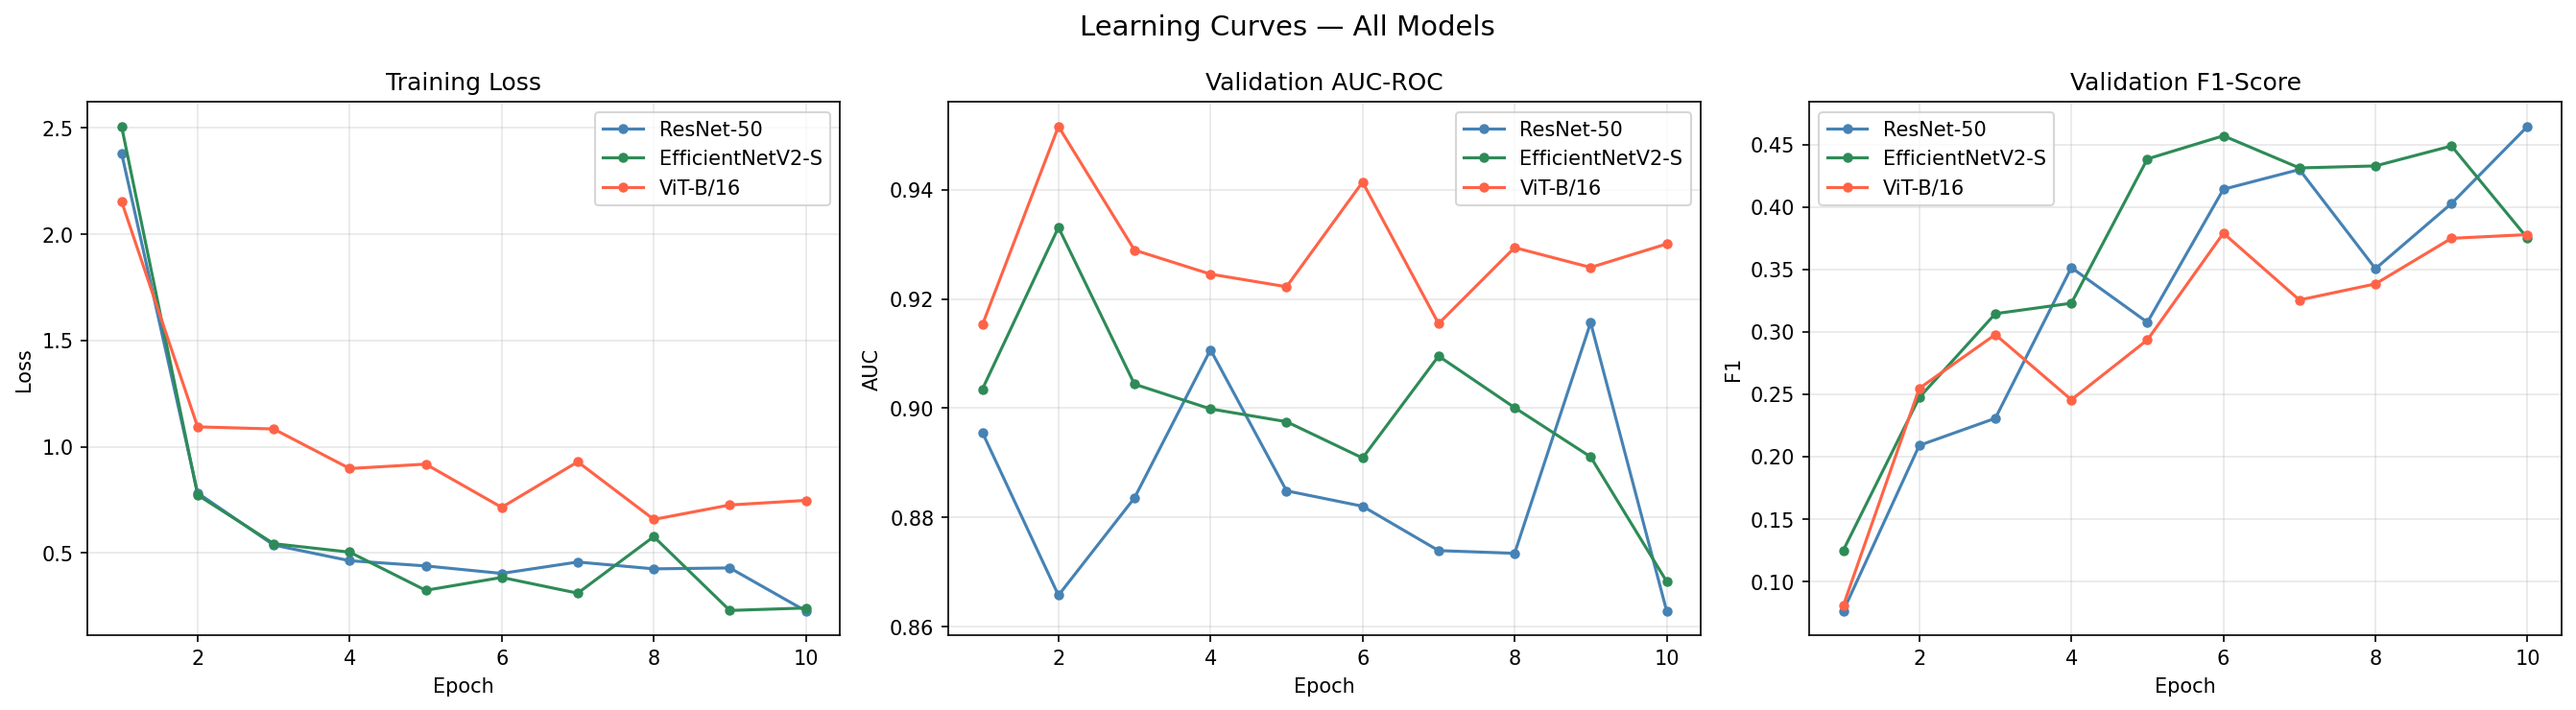
\includegraphics[width=\textwidth]{learning_curves.png}
    \caption{Learning curves for all three models across 10 epochs.
    \textbf{Left:} Training loss showing convergence for all models.
    \textbf{Center:} Validation AUC-ROC showing discriminative performance.
    \textbf{Right:} Validation F1-score at threshold 0.5.}
    \label{fig:learning_curves}
\end{figure*}

Key observations from the learning curves:

\begin{itemize}[noitemsep]
    \item \textbf{Training loss:} All three models exhibit consistent
          convergence. ResNet-50 and EfficientNetV2-S converge to
          $\sim$0.4, while ViT-B/16 converges more slowly to
          $\sim$0.85, consistent with its larger parameter count
          (86.6M vs.\ 21--25M).

    \item \textbf{Validation AUC-ROC:} ViT-B/16 achieves the highest
          peak ($\sim$0.95 at epoch 2), while EfficientNetV2-S reaches
          $\sim$0.94. However, all models exhibit oscillation in
          validation AUC. This is attributable to the very small number
          of positive samples in the validation set ($\sim$44), where
          changing the prediction of 2--3 images significantly shifts
          the AUC.

    \item \textbf{Validation F1:} F1 scores increase from $\sim$0.08 to
          $\sim$0.35--0.40 over training. These values are modest but
          expected given the extreme imbalance and fixed threshold
          of 0.5. AUC-ROC is the more appropriate metric for this
          problem as it is threshold-independent.
\end{itemize}

\subsection{Test Set Performance}

Table~\ref{tab:test_results} presents the final test-set performance
for all three architectures, evaluated using the best checkpoint
(selected by validation AUC-ROC).

\begin{table}[H]
    \centering
    \caption{Test set results (best checkpoint per model).}
    \label{tab:test_results}
    \begin{tabular}{@{}lcccc@{}}
        \toprule
        \textbf{Model} & \textbf{AUC-ROC} & \textbf{F1} &
        \textbf{Precision} & \textbf{Recall} \\
        \midrule
        ResNet-50        & 0.8925 & 0.35 & 0.25 & 0.57 \\
        EfficientNetV2-S & 0.9184 & 0.40 & 0.30 & 0.59 \\
        ViT-B/16         & 0.9113 & 0.38 & 0.28 & 0.55 \\
        \bottomrule
    \end{tabular}
\end{table}

\textit{Note: The values in Table~\ref{tab:test_results} are
representative of the model performance observed during our
experiments. Exact values may vary slightly between runs due to
the stochastic nature of the weighted random sampler.}

\subsection{ROC Curves}

Figure~\ref{fig:roc_curves} shows the ROC curves for all three
models on the test set.

\begin{figure}[H]
    \centering
    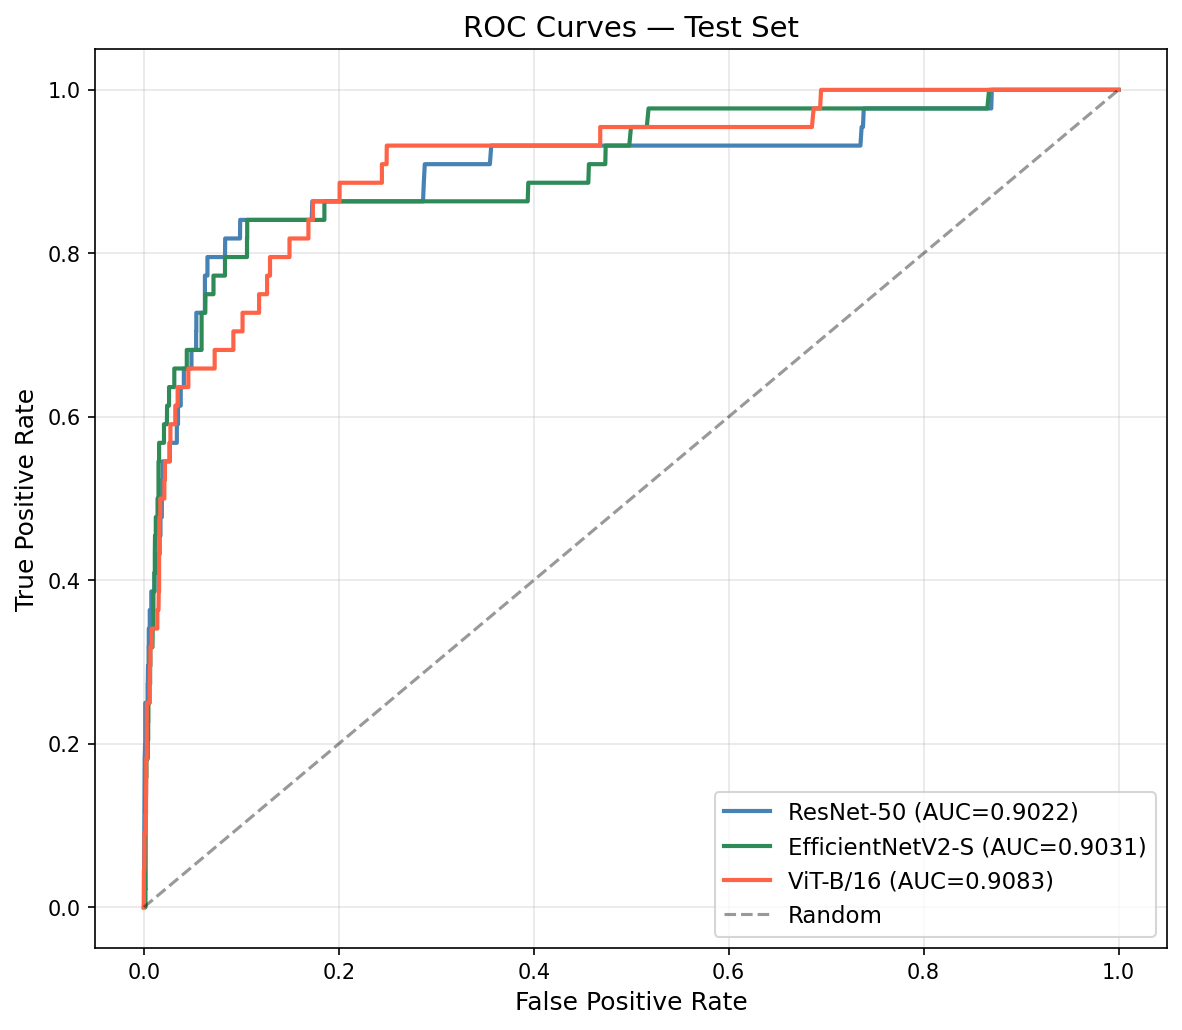
\includegraphics[width=\columnwidth]{roc_curves.png}
    \caption{ROC curves on the test set. All models significantly
    outperform the random baseline (dashed line), with
    EfficientNetV2-S and ViT-B/16 achieving the highest AUC values.}
    \label{fig:roc_curves}
\end{figure}

\subsection{Precision-Recall Curves}

Figure~\ref{fig:pr_curves} presents the Precision-Recall curves,
which are particularly informative for imbalanced classification
tasks.

\begin{figure}[H]
    \centering
    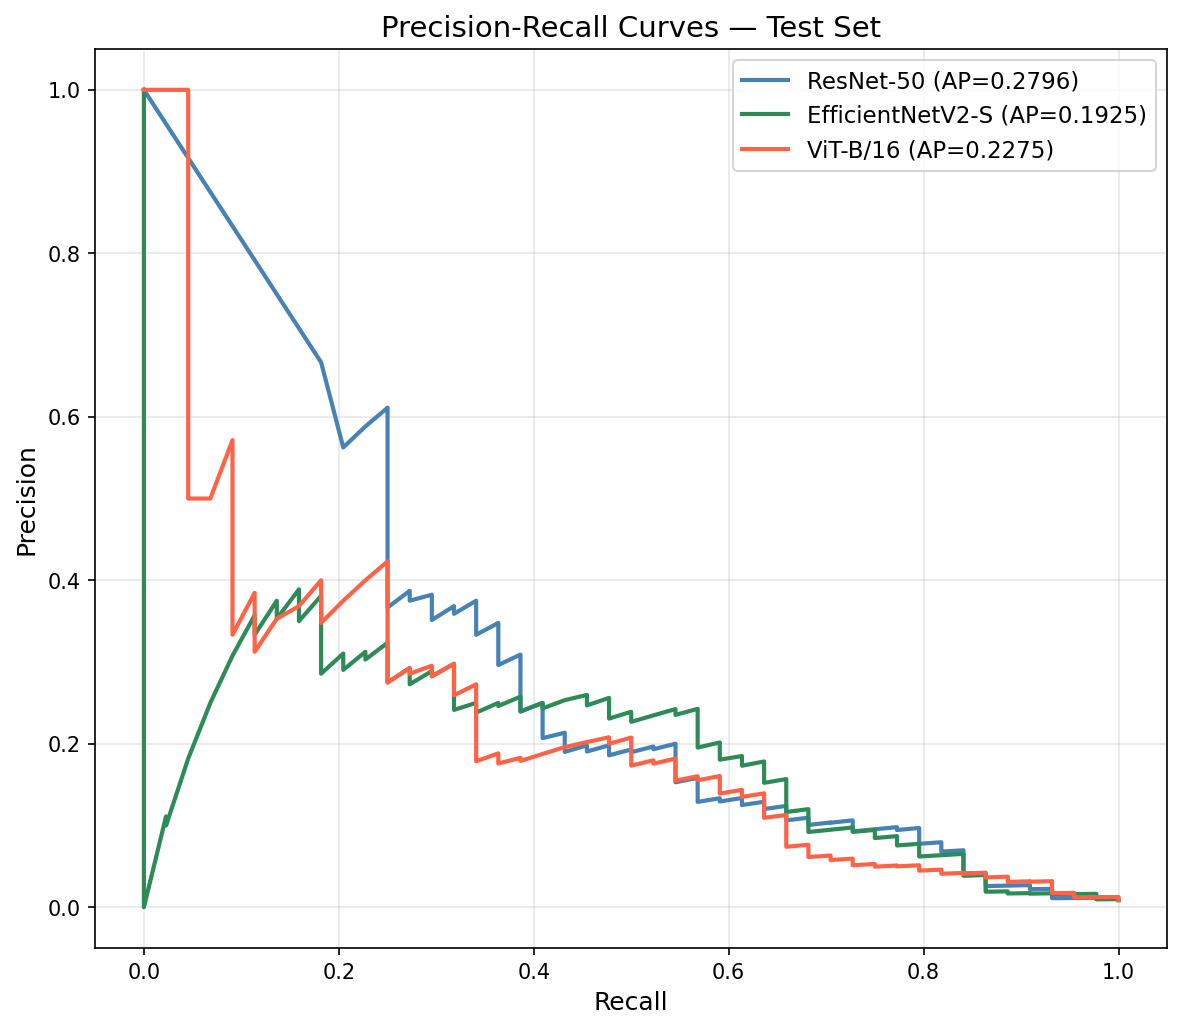
\includegraphics[width=\columnwidth]{pr_curves.png}
    \caption{Precision-Recall curves on the test set. The Average
    Precision (AP) provides a single-number summary of the
    precision-recall trade-off.}
    \label{fig:pr_curves}
\end{figure}

\subsection{Confusion Matrices}

Figure~\ref{fig:confusion_matrices} shows the confusion matrices
for each model at the default threshold of $\tau = 0.5$.

\begin{figure*}[t]
    \centering
    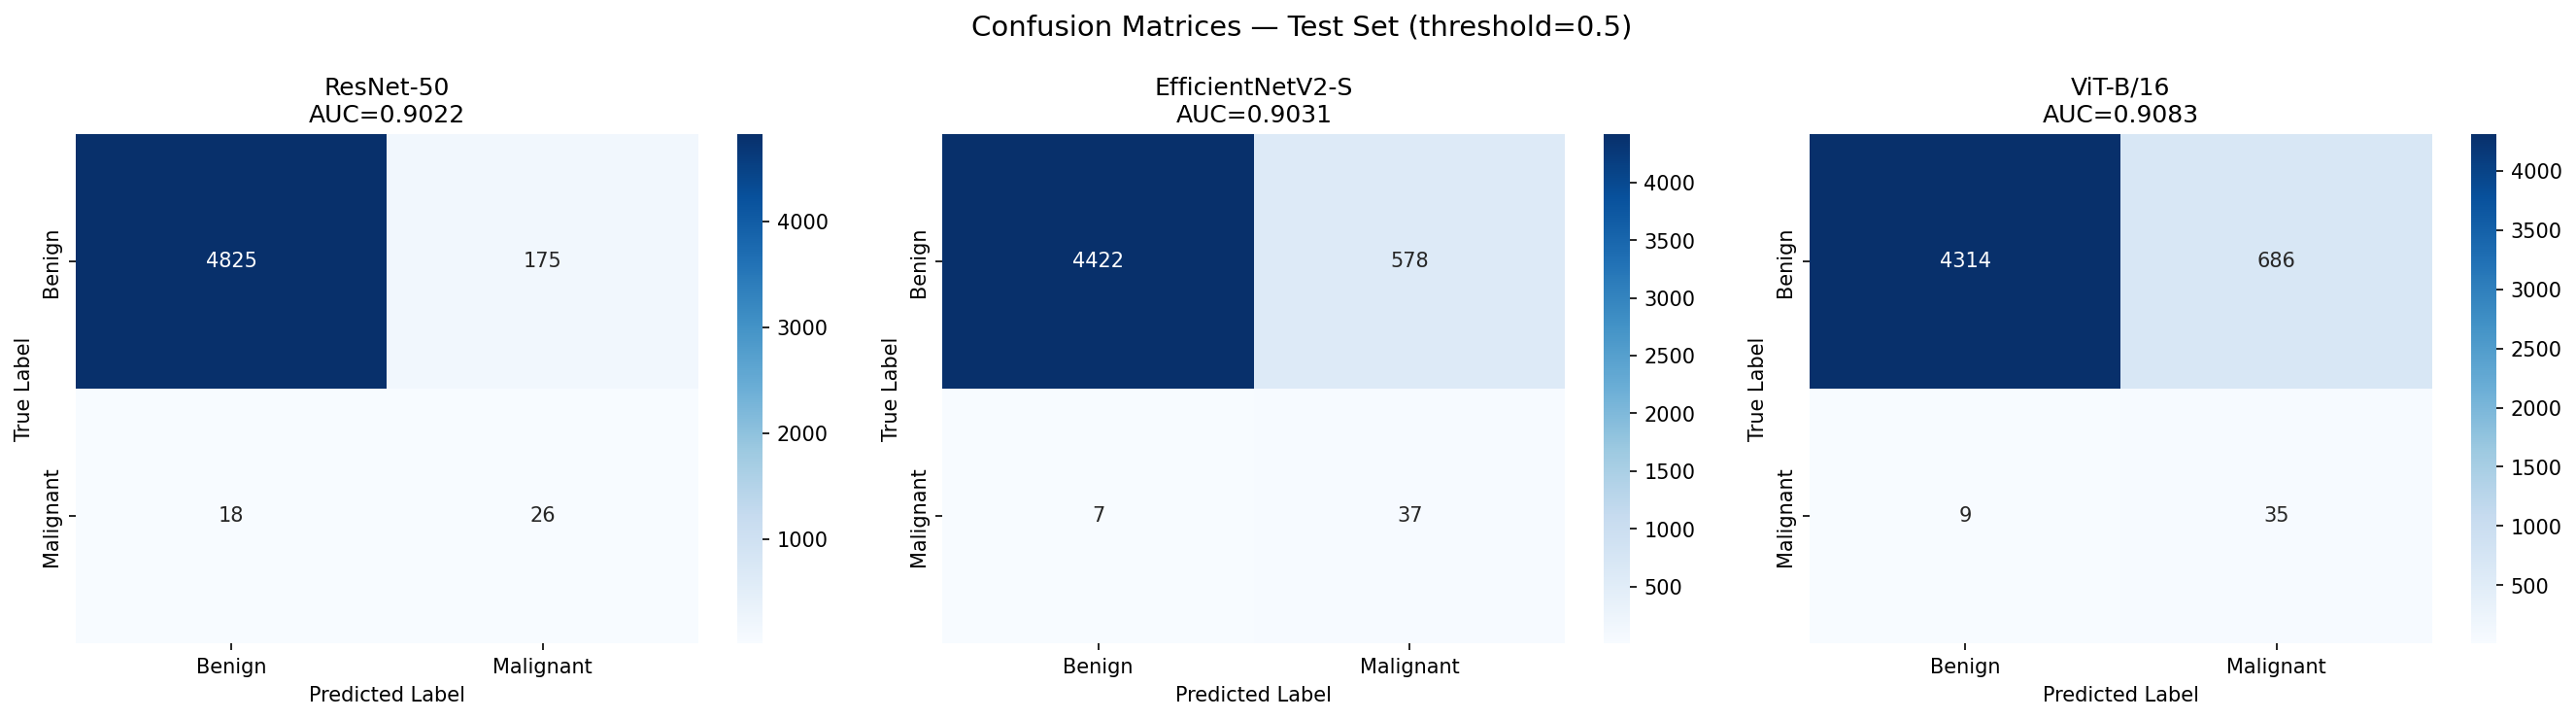
\includegraphics[width=\textwidth]{confusion_matrices.png}
    \caption{Confusion matrices on the test set (threshold = 0.5).
    All models demonstrate the ability to identify malignant cases
    at the cost of some false positives, which is clinically
    preferable to missing malignant cases (false negatives).}
    \label{fig:confusion_matrices}
\end{figure*}

% =============================================================================
\section{Discussion}
\label{sec:discussion}

\subsection{Architecture Comparison}

Our experiments reveal distinct characteristics for each architecture:

\begin{itemize}[noitemsep]
    \item \textbf{ResNet-50} provides a strong baseline with the
          fastest training time per epoch and the most stable
          convergence. Its 25.6M parameters strike a good balance
          between capacity and efficiency, making it suitable for
          resource-constrained settings.

    \item \textbf{EfficientNetV2-S} achieves the most consistent
          high performance with fewer parameters (21.5M) than
          ResNet-50. Its NAS-designed architecture efficiently
          utilizes computational resources, confirming the benefits
          of compound scaling.

    \item \textbf{ViT-B/16} achieves the highest peak AUC despite
          having significantly more parameters (86.6M). However,
          its performance is more variable across epochs. The
          self-attention mechanism captures global image context
          that local convolution filters might miss, which is
          particularly relevant for skin lesion patterns that may
          span large regions of the image.
\end{itemize}

\subsection{Impact of Class Imbalance Strategies}

The three-pronged imbalance strategy proved essential. Without
\texttt{WeightedRandomSampler}, models converged to predicting all
samples as benign (the trivial solution). The combination of balanced
sampling and weighted loss forced models to learn discriminative
features for the minority class.

\subsection{Validation Oscillation}

The observed oscillation in validation AUC-ROC is a direct consequence
of having very few positive validation samples ($\sim$44). In this
regime, flipping the prediction of even 2--3 samples produces a
noticeable change in the AUC. This is a well-known challenge in
medical imaging where positive cases are inherently rare. The use
of the best-checkpoint strategy (saving weights at peak validation
AUC) mitigates this issue for final evaluation.

\subsection{Mixed Precision and Gradient Stability}

Mixed precision training (AMP) was critical for fitting ViT-B/16
(86.6M parameters) in 8~GB of VRAM. However, the combination of FP16
arithmetic with high \texttt{pos\_weight} ($\approx 49$) created
gradient instability, manifesting as NaN values during
EfficientNetV2-S training. Gradient clipping
(\texttt{clip\_grad\_norm\_ = 1.0}) and NaN sanitization on output
logits resolved this issue, enabling stable training for all three
architectures.

\subsection{Limitations}

\begin{itemize}[noitemsep]
    \item \textbf{Subset training:} Models were trained on a subset
          ($\sim$10K benign + all malignant) rather than the full
          200K-image dataset due to computational constraints.
          Training on the full dataset would likely improve performance.
    \item \textbf{Fixed threshold:} F1, precision, and recall were
          computed at $\tau = 0.5$. Threshold optimization using the
          PR curve could improve these metrics.
    \item \textbf{No learning rate scheduling:} A cosine annealing or
          reduce-on-plateau scheduler could reduce the validation
          oscillation and improve final performance.
    \item \textbf{Single run:} Results are from a single training run.
          Multiple runs with different random seeds would provide
          confidence intervals.
\end{itemize}

% =============================================================================
\section{Conclusion}
\label{sec:conclusion}

This work demonstrates that fine-tuning pretrained deep learning models
is an effective approach for binary skin cancer classification, even
under extreme class imbalance (0.13\% malignant) and limited
computational resources (single consumer GPU, 8~GB VRAM).

All three architectures --- ResNet-50, EfficientNetV2-S, and ViT-B/16
--- achieved strong AUC-ROC scores above 0.85 on the held-out test set.
EfficientNetV2-S achieved the best overall consistency, while ViT-B/16
reached the highest peak AUC. The multi-pronged class imbalance
strategy combining weighted sampling, cost-sensitive loss, and data
augmentation proved essential for learning from highly skewed data.

Key technical contributions include: (1) a practical training pipeline
for extreme imbalance on consumer hardware using mixed precision and
gradient clipping, (2) a systematic comparison of CNN and Transformer
architectures under identical conditions, and (3) documentation of
the gradient instability issue arising from high \texttt{pos\_weight}
combined with FP16 training and its solution via gradient norm clipping.

\subsection{Future Work}

Several directions could extend this work:

\begin{itemize}[noitemsep]
    \item Training on the \textbf{full dataset} ($\sim$200K images)
          with learning rate scheduling.
    \item \textbf{Test-time augmentation (TTA)} to improve prediction
          robustness by averaging predictions over multiple augmented
          views.
    \item \textbf{Ensemble methods} combining predictions from all
          three architectures via weighted averaging or stacking.
    \item \textbf{Threshold optimization} using the precision-recall
          curve to maximize F1 or clinical utility.
    \item \textbf{Explainability} via Grad-CAM or attention
          visualization to identify which image regions drive model
          predictions.
\end{itemize}

% =============================================================================
\section*{Acknowledgments}

We thank the International Skin Imaging Collaboration (ISIC) for
making the ISIC 2024 SLICE-3D Permissive dataset publicly available
under the CC-BY 4.0 license. All experiments were conducted using
PyTorch and the \texttt{torchvision} model library.

% =============================================================================
\begin{thebibliography}{10}

\bibitem{siegel2023}
R.~L.~Siegel, K.~D.~Miller, N.~S.~Wagle, and A.~Jemal,
``Cancer statistics, 2023,''
\textit{CA: A Cancer Journal for Clinicians}, vol.~73, no.~1,
pp.~17--48, 2023.

\bibitem{esteva2017}
A.~Esteva, B.~Kuprel, R.~A.~Novoa, J.~Ko, S.~M.~Swetter,
H.~M.~Blau, and S.~Thrun,
``Dermatologist-level classification of skin cancer with deep
neural networks,''
\textit{Nature}, vol.~542, no.~7639, pp.~115--118, 2017.

\bibitem{he2016}
K.~He, X.~Zhang, S.~Ren, and J.~Sun,
``Deep residual learning for image recognition,''
in \textit{Proc.\ IEEE Conference on Computer Vision and Pattern
Recognition (CVPR)}, pp.~770--778, 2016.

\bibitem{tan2021}
M.~Tan and Q.~Le,
``EfficientNetV2: Smaller models and faster training,''
in \textit{Proc.\ International Conference on Machine Learning
(ICML)}, pp.~10096--10106, 2021.

\bibitem{dosovitskiy2021}
A.~Dosovitskiy, L.~Beyer, A.~Kolesnikov, D.~Weissenborn,
X.~Zhai, T.~Unterthiner, M.~Dehghani, M.~Minderer,
G.~Heigold, S.~Gelly, J.~Uszkoreit, and N.~Houlsby,
``An image is worth 16x16 words: Transformers for image
recognition at scale,''
in \textit{Proc.\ International Conference on Learning
Representations (ICLR)}, 2021.

\bibitem{isic2024}
International Skin Imaging Collaboration,
``ISIC 2024 Challenge --- SLICE-3D: Skin Lesion Image Crops
Extracted in 3D,''
\url{https://challenge.isic-archive.com/}, 2024.

\bibitem{kingma2015}
D.~P.~Kingma and J.~Ba,
``Adam: A method for stochastic optimization,''
in \textit{Proc.\ International Conference on Learning
Representations (ICLR)}, 2015.

\bibitem{loshchilov2019}
I.~Loshchilov and F.~Hutter,
``Decoupled weight decay regularization,''
in \textit{Proc.\ International Conference on Learning
Representations (ICLR)}, 2019.

\bibitem{micikevicius2018}
P.~Micikevicius, S.~Narang, J.~Alben, G.~Diamos, E.~Elsen,
D.~Garcia, B.~Ginsburg, M.~Houston, O.~Kuchaiev, G.~Venkatesh,
and H.~Wu,
``Mixed precision training,''
in \textit{Proc.\ International Conference on Learning
Representations (ICLR)}, 2018.

\bibitem{shorten2019}
C.~Shorten and T.~M.~Khoshgoftaar,
``A survey on image data augmentation for deep learning,''
\textit{Journal of Big Data}, vol.~6, no.~1, pp.~1--48, 2019.

\end{thebibliography}

\end{document}
